\documentclass[11pt]{article}

\usepackage{nmrdoc}
\usepackage{siunitx}
\usepackage{bm}
\usepackage{tikz}

\sisetup{per-mode=symbol}
\DeclareSIUnit{\angstrom}{\text{\AA}}

\newcommand{\code}[1]{\texttt{#1}}
\setlength{\parindent}{0pt}
\setlength{\parskip}{0.42em}
\emergencystretch=2em

\begin{document}
\NmrTitle{Numerical Addendum: WaterField Calculator}

WaterField is a finite real-space point-charge sum followed by a trace
projection. For each protein atom it scans explicit waters, keeps waters whose
oxygen lies inside or on the configured cutoff, and evaluates the three water
charge sites for addition to a vector field and an electric-field-gradient
tensor. There is no Ewald, PME, reciprocal-space, or dielectric-reaction term in
this calculator; the cutoff sum is the whole electrostatics for this result.
The listings below are distilled from the source --- loops and bookkeeping
trimmed --- but the constants, guards, inequalities, and arithmetic are the
implementation's.

\section{The real-space cutoff}

The current \code{WaterFieldResult::Compute} path does not query a water
k-d tree. The class declares \code{SpatialIndexResult} as a dependency, and the
solvent object carries \code{water\_O\_positions}, but this function scans
\code{solvent.waters[0..W)} for each of the \(N\) protein atoms. The oxygen
cutoff reduces the number of charge sites accumulated, not the number of water
records visited, so the scan is \(O(NW)\) before the three-site charge work.

The gate is oxygen-based. With target atom position \(\bm x_i\), water oxygen
position \(\bm s_{wO}\), and
\(r_c=\code{water\_efield\_cutoff}=\SI{15.0}{\angstrom}\), the code omits a
water only when
\[
  |\bm s_{wO}-\bm x_i|^2 > r_c^2 .
\]
Equality at the cutoff is kept. Once a water passes, all three charge sites
\((O,H1,H2)\) are evaluated with their own charge-site vectors. A hydrogen can
therefore be included because its oxygen passed the gate; the code does not run
a separate hydrogen cutoff.

\begin{codebox}
double rc  = cfg("water_efield_cutoff");        // 15.0 A
double r1  = cfg("water_first_shell_cutoff");   //  3.5 A
double r2  = cfg("water_second_shell_cutoff");  //  5.5 A
double rc2 = rc * rc, r1sq = r1 * r1, r2sq = r2 * r2;

for (size_t wi = 0; wi < W; ++wi) {             // scans all waters
    const auto& water = solvent.waters[wi];
    Vec3 rO = water.O_pos - pos_i;
    double dO2 = rO.squaredNorm();
    if (dO2 > rc2) continue;                    // equality is kept

    bool first = (dO2 < r1sq);
    if (first)      ++n_first;                  // O distance < 3.5 A
    else if (dO2 < r2sq) ++n_second;            // 3.5 A <= O < 5.5 A

    add_charge(water.O_pos,  water.O_charge);
    add_charge(water.H1_pos, water.H_charge);
    add_charge(water.H2_pos, water.H_charge);
}
\end{codebox}

The shell tests are counts and accumulation gates, not separate electrostatic
models. \code{n\_first} counts waters with oxygen distance
\(<\SI{3.5}{\angstrom}\). \code{n\_second} counts waters that failed the first
test and have oxygen distance \(<\SI{5.5}{\angstrom}\). The first-shell field
and EFG accumulators receive the same three charge-site contributions as the
total accumulators, but only for waters whose oxygen is in the first shell.
The second shell is a count only.

\begin{figure}[ht]
\centering
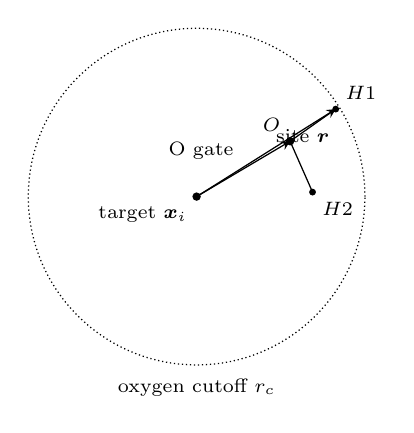
\begin{tikzpicture}[scale=0.95,line width=0.45pt,>=stealth]
  \coordinate (T) at (0,0);
  \coordinate (O) at (1.25,0.74);
  \coordinate (H1) at (1.86,1.17);
  \coordinate (H2) at (1.55,0.06);

  \draw[densely dotted] (T) circle (2.25);
  \node at (0,-2.55) {\scriptsize oxygen cutoff \(r_c\)};

  \fill (T) circle (1.6pt) node[below left] {\scriptsize target \(\bm x_i\)};
  \draw (O) -- (H1);
  \draw (O) -- (H2);
  \fill (O) circle (1.6pt) node[above left] {\scriptsize \(O\)};
  \fill (H1) circle (1.3pt) node[above right] {\scriptsize \(H1\)};
  \fill (H2) circle (1.3pt) node[below right] {\scriptsize \(H2\)};

  \draw[->] (T) -- (O) node[midway,above left] {\scriptsize O gate};
  \draw[->] (T) -- (H1) node[midway,above right] {\scriptsize site \(\bm r\)};
\end{tikzpicture}
\caption{The oxygen position decides whether the water molecule enters the
sum. Once it enters, all three charge sites use their own target-to-site vector
\(\bm r\) in the Coulomb kernels.}
\end{figure}

The cutoff is an omission, not a switching function. A water outside the oxygen
cutoff contributes no field, no EFG, and no long-range correction. Nothing is
added later to represent the missing real-space tail or a reciprocal-space
counterpart.

\section{One charge contribution}

For a charge site from an accepted water, \code{q\_pos} is \(\bm s_j\),
\code{q} is the site charge in elementary-charge units, and \code{r} is
\[
  \bm r = \bm s_j-\bm x_i ,
\]
the vector from the target atom to the water charge site. The code forms
\(r^2=|\bm r|^2\), \(r=|\bm r|\), \(r^3\), and \(r^5\) from that vector. Before
the divisions, it passes \(|\bm r|\) through the shared
\code{MinDistanceFilter}. The filter accepts
\(|\bm r|\ge\SI{0.1}{\angstrom}\); a closer site increments the per-atom
rejection count and contributes nothing. The rejected term is dropped, not
evaluated at a floor distance of \(\SI{0.1}{\angstrom}\) and not reweighted into
another term.

\begin{codebox}
auto add_charge = [&](const Vec3& q_pos, double q) {
    Vec3 r = q_pos - pos_i;              // target -> charge site
    double r_sq = r.squaredNorm();
    double r_mag = std::sqrt(r_sq);

    KernelEvaluationContext ctx;
    ctx.atom_index = ai;
    ctx.distance = r_mag;
    if (!filters.AcceptAll(ctx)) { ++n_singularity_guard; return; }

    double r3 = r_sq * r_mag;
    double r5 = r3 * r_sq;

    Vec3 E_j = (COULOMB_KE * q / r3) * r;
    Mat3 V_j = COULOMB_KE * q *
        (3.0 * r * r.transpose() / r5 - Mat3::Identity() / r3);

    E_total += E_j;      V_total += V_j;
    if (first) { E_first += E_j; V_first += V_j; }
};
\end{codebox}

\code{COULOMB\_KE} is \(\SI{14.3996}{\volt\angstrom}\). With charges in \(e\)
and distances in \(\si{\angstrom}\), \code{E\_j} lands in
\(\si{\volt\per\angstrom}\) and \code{V\_j} lands in
\(\si{\volt\per\square\angstrom}\). The vector contribution points along
\(\bm r\) for a positive charge and opposite \(\bm r\) for a negative charge.
The displacement \(\bm r\) here runs from the field atom to the water charge
(\code{q\_pos}\,$-$\,\code{pos\_i}), the reverse of the textbook source-to-field
direction; the field signs below follow that convention.
The tensor contribution is the point-charge Hessian:
\[
  V^{(j)}_{ab} =
  k_e q_j\left(
    \frac{3 r_a r_b}{r^5} - \frac{\delta_{ab}}{r^3}
  \right).
\]
Along the charge-site direction a positive charge contributes \(+2k_eq_j/r^3\);
in each transverse direction it contributes \(-k_eq_j/r^3\). A negative charge
reverses those signs. The outer product \(r_ar_b\) is symmetric and the identity
term is symmetric, so each accepted source adds a symmetric matrix to
\code{V\_total}; the code does not create an antisymmetric EFG term.

\section{Trace projection and guards}

Each source tensor above is traceless in exact arithmetic:
\[
  \operatorname{tr}\bm V^{(j)}
  = k_e q_j\left(\frac{3(r_x^2+r_y^2+r_z^2)}{r^5}
                 -\frac{3}{r^3}\right)=0 .
\]
The exact finite sum is therefore traceless. Floating-point arithmetic
does not preserve that identity term by term: the products, divisions, and
additions are rounded, and many rounded terms are accumulated into the same
three diagonal entries. Before decomposition, the code subtracts one third of
the accumulated trace from each diagonal entry. This projection changes only
the EFG diagonal. It leaves the off-diagonal EFG entries and the vector fields
unchanged.

There is no explicit \(\frac12(V+V^{\mathsf T})\) call in this source. The EFG
is symmetric by construction from \(r r^{\mathsf T}\) and \(\bm I\), and the
only tensor projection applied here is the trace projection shown below. There
is also no WaterField \code{std::isfinite} sanitizer for the vector or EFG
matrices. The distance filter prevents the small-\(r\) divisions from running
below \SI{0.1}{\angstrom}; it is not a matrix finite-value pass.

\begin{codebox}
double trace_total = V_total.trace() / 3.0;
V_total -= trace_total * Mat3::Identity();

double trace_first = V_first.trace() / 3.0;
V_first -= trace_first * Mat3::Identity();

double E_mag = E_total.norm();
if (E_mag > cfg("efield_magnitude_sanity_clamp")) {   // 100.0 V/A
    double scale = cfg("efield_magnitude_sanity_clamp") / E_mag;
    E_total *= scale;
    E_first *= scale;
}
\end{codebox}

The magnitude clamp is a vector-field guard only. For a finite vector with
\(|\code{E\_total}|>\SI{100.0}{\volt\per\angstrom}\), the code multiplies
\code{E\_total} and \code{E\_first} by
\(\SI{100.0}{\volt\per\angstrom}/|\code{E\_total}|\). In exact arithmetic this
sets the total-vector magnitude to \(\SI{100.0}{\volt\per\angstrom}\) and keeps
its direction. The first-shell vector receives the same scale factor, even
though the test was made on the total vector. The EFG tensors are not scaled by
this clamp.

\section{Shared tensor split}

After the trace projection, \code{V\_total} and \code{V\_first} pass through
\code{SphericalTensor::Decompose}. The decomposition is closed-form arithmetic
on the input matrix \code{sigma}, not an eigensolve. The trace average gives
\(T_0\), the antisymmetric part gives the three \(T_1\) components, and the
symmetric traceless part gives the five \(T_2\) components.

\begin{codebox}
st.T0 = sigma.trace() / 3.0;

st.T1[0] = 0.5 * (sigma(1,2) - sigma(2,1));
st.T1[1] = 0.5 * (sigma(2,0) - sigma(0,2));
st.T1[2] = 0.5 * (sigma(0,1) - sigma(1,0));

double Sxx = sigma(0,0) - st.T0;
double Syy = sigma(1,1) - st.T0;
double Szz = sigma(2,2) - st.T0;
double Sxy = 0.5 * (sigma(0,1) + sigma(1,0));
double Sxz = 0.5 * (sigma(0,2) + sigma(2,0));
double Syz = 0.5 * (sigma(1,2) + sigma(2,1));

st.T2[0] = std::sqrt(2.0) * Sxy;
st.T2[1] = std::sqrt(2.0) * Syz;
st.T2[2] = std::sqrt(3.0 / 2.0) * Szz;
st.T2[3] = std::sqrt(2.0) * Sxz;
st.T2[4] = (Sxx - Syy) / std::sqrt(2.0);
\end{codebox}

The \(T_2\) constants make the five-vector isometric with the symmetric
traceless matrix \(\bm S\). An off-diagonal entry such as \(S_{xy}\) appears
twice in the matrix, so it contributes \(2S_{xy}^2\) to the Frobenius sum; the
stored \(\sqrt2\,S_{xy}\) squares to the same amount. The diagonal pair
\(\sqrt{3/2}\,S_{zz}\) and \((S_{xx}-S_{yy})/\sqrt2\) carries the two diagonal
degrees of freedom after the trace part is removed.

For WaterField, the matrix entering \code{Decompose} has been trace-projected
and is symmetric by construction. Its \(T_0\) channel carries only roundoff left
after the trace projection, if any; its \(T_1\) channel vanishes when the
antisymmetric part is zero. \code{WriteFeatures} emits neither: \code{PackT2}
writes only the five \(T_2\) entries for \code{water\_efg.npy} and
\code{water\_efg\_first.npy}, each with shape \(N\times5\).

\section{Glossary}

\textbf{Oxygen cutoff.} The target atom carries a sphere around it, but the
water molecule is admitted or omitted by the oxygen point alone. A water at
exactly \(\SI{15.0}{\angstrom}\) oxygen distance is kept because the code
rejects only \(d_O^2>r_c^2\); a water at exactly \(\SI{3.5}{\angstrom}\) is
counted in the second shell, and a water at exactly
\(\SI{5.5}{\angstrom}\) is not counted in either shell. Formally, the summed
water set is \(\{w:|\bm s_{wO}-\bm x_i|\le r_c\}\). The first-shell label uses
\(d_O<r_1\), and the second-shell label uses \(r_1\le d_O<r_2\).

\textbf{Point-charge EFG kernel.} The point-charge potential has one sign of
curvature along the source-target line and the opposite sign in the two
transverse directions. For a positive charge on the \(x\)-axis, the Cartesian
tensor is proportional to \(\operatorname{diag}(2,-1,-1)\); the three diagonal
entries sum to zero. Formally, the kernel is
\(k_eq(3r_ar_b/r^5-\delta_{ab}/r^3)\), the Hessian of the point-charge
potential away from the source.

\textbf{Traceless projection.} Sharing the diagonal's leftover sum back out
evenly: subtract one third of the current trace from each diagonal entry so the
three again add to zero, off-diagonal entries untouched. If the accumulated
diagonal is \((2+\epsilon,-1,-1)\), the projection subtracts \(\epsilon/3\) from
each diagonal entry and restores zero trace in exact arithmetic. Formally, it
maps \(V\) to \(V-\frac13\operatorname{tr}(V)\bm I\).

\textbf{Spherical tensor split.} A \(3\times3\) tensor holds three kinds of
content that rotate without mixing --- an orientation-free size (the scalar
trace, \(T_0\)), an axial twist from its antisymmetric part (the three \(T_1\)
components), and a five-number traceless shape for the rest of the
direction-dependence (the five \(T_2\) components). WaterField's EFG output
writes only the five \(T_2\) components because the input tensor is symmetric and
trace-projected before decomposition. Formally, it is the closed-form split of a
\(3\times3\) tensor's nine components into dimensions \(1+3+5\), with the \(T_2\)
basis normalized to preserve the Frobenius norm.

\end{document}
